% !TEX root = ../main.tex
% File: chapters_part1/chap2_3.tex
% Nội dung cho Phần 2.3: Các thuật toán Học máy Thống kê

\section{Các thuật toán Học máy Thống kê}
\label{sec:statistical_ml_algos}

Sau khi đã biến đổi văn bản thành các vector số (sử dụng BoW hoặc TF-IDF), chúng ta đã sẵn sàng để "dạy" cho máy tính. Các thuật toán học máy thống kê là những công cụ cho phép chúng ta xây dựng các mô hình có khả năng học các mẫu (patterns) từ dữ liệu đã được gán nhãn, và sau đó sử dụng các mẫu đó để đưa ra dự đoán trên dữ liệu mới.

Mục này sẽ giới thiệu một số thuật toán kinh điển đã tạo nên xương sống của NLP trong kỷ nguyên thống kê. Chúng được chia thành hai nhóm chính: các mô hình cho bài toán \textbf{phân loại} và các mô hình cho bài toán \textbf{học chuỗi}.

\subsection{Các mô hình Phân loại (Classification Models)}
\label{ssec:classification_models}
Đây là nhóm các thuật toán dùng để giải quyết các bài toán phân loại văn bản, ví dụ như phân tích cảm xúc (tích cực/tiêu cực), phân loại chủ đề tin tức, phát hiện thư rác.

\subsubsection{Naive Bayes}
Naive Bayes là một trong những thuật toán phân loại đơn giản, nhanh và đáng ngạc nhiên là rất hiệu quả cho các tác vụ văn bản \cite{manning2008introduction}.

\paragraph{Trực giác cốt lõi}
Thuật toán này dựa trên \textbf{Định lý Bayes}. Để phân loại một tài liệu $d$ vào một lớp $c$ (ví dụ: `spam` hoặc `not-spam`), Naive Bayes tính toán xác suất của mỗi lớp khi biết tài liệu đó, $P(c|d)$, và chọn lớp có xác suất cao nhất.

Sử dụng định lý Bayes, ta có:
$$ P(c|d) = \frac{P(d|c) \cdot P(c)}{P(d)} $$
Trong đó:
\begin{itemize}
    \item $P(c|d)$: Xác suất hậu nghiệm (posterior) - xác suất của lớp $c$ khi biết tài liệu $d$. Đây là thứ chúng ta muốn tìm.
    \item $P(d|c)$: Xác suất khả năng (likelihood) - xác suất của tài liệu $d$ khi biết nó thuộc lớp $c$.
    \item $P(c)$: Xác suất tiên nghiệm (prior) - xác suất của lớp $c$ trong toàn bộ dữ liệu.
    \item $P(d)$: Xác suất của tài liệu $d$. Vì $P(d)$ là hằng số đối với tất cả các lớp, chúng ta có thể bỏ qua nó khi so sánh các lớp với nhau.
\end{itemize}
Do đó, việc tối đa hóa $P(c|d)$ tương đương với việc tối đa hóa $P(d|c) \cdot P(c)$.

\paragraph{Giả định "Ngây thơ" (The "Naive" Assumption)}
Để tính $P(d|c) = P(w_1, w_2, \dots, w_n | c)$, Naive Bayes đưa ra một giả định rất mạnh và "ngây thơ" (naive): \textbf{các từ (đặc trưng) trong tài liệu là độc lập có điều kiện với nhau khi biết lớp $c$}.
$$ P(d|c) = P(w_1, w_2, \dots, w_n | c) \approx \prod_{i=1}^{n} P(w_i | c) $$
Mặc dù giả định này rõ ràng là sai trong thực tế (trật tự từ và sự phụ thuộc giữa các từ là rất quan trọng), nó giúp việc tính toán trở nên cực kỳ đơn giản và hiệu quả.

\paragraph{Công thức cuối cùng}
Lớp $\hat{c}$ được dự đoán cho tài liệu $d$ là:
\begin{equation}
    \hat{c} = \underset{c \in C}{\arg\max} \left( P(c) \cdot \prod_{i=1}^{n} P(w_i | c) \right)
    \label{eq:naive_bayes}
\end{equation}
Trong thực tế, do tích của nhiều xác suất nhỏ có thể dẫn đến sai số làm tròn, người ta thường tính toán trên logarit:
$$ \hat{c} = \underset{c \in C}{\arg\max} \left( \log P(c) + \sum_{i=1}^{n} \log P(w_i | c) \right) $$
Các xác suất $P(c)$ và $P(w_i|c)$ được học từ tập dữ liệu huấn luyện bằng cách đếm tần suất và sử dụng kỹ thuật làm mịn (ví dụ: Laplace) để tránh xác suất zero.

\begin{tcolorbox}[
    title=Đánh giá Naive Bayes,
    colback=blue!5!white, colframe=blue!50!black, fonttitle=\bfseries
]
\textbf{Ưu điểm:}
\begin{itemize}
    \item \textbf{Cực kỳ nhanh:} Cả quá trình huấn luyện và dự đoán đều chỉ là các phép đếm và nhân/cộng, rất hiệu quả.
    \item \textbf{Cần ít dữ liệu huấn luyện:} Hoạt động tương đối tốt ngay cả với dữ liệu nhỏ.
    \item \textbf{Mô hình diễn giải được:} Có thể kiểm tra xác suất $P(w|c)$ để xem từ nào đóng góp nhiều nhất vào việc phân loại một lớp.
\end{itemize}
\textbf{Nhược điểm:}
\begin{itemize}
    \item \textbf{Giả định độc lập "ngây thơ":} Không thể nắm bắt mối quan hệ và trật tự từ, làm hạn chế hiệu năng ở các bài toán phức tạp.
\end{itemize}
\end{tcolorbox}


\subsubsection{Hồi quy Logistic (Logistic Regression)}
Hồi quy Logistic \cite{hosmer2013applied}, mặc dù tên gọi có chữ "hồi quy", lại là một thuật toán phân loại mạnh mẽ và được sử dụng cực kỳ rộng rãi. Nó thuộc nhóm các mô hình \textbf{phân biệt (discriminative models)}, trái ngược với Naive Bayes là một mô hình \textbf{sinh (generative model)}.

\paragraph{Trực giác cốt lõi}
Thay vì mô hình hóa $P(d|c)$ như Naive Bayes, Hồi quy Logistic mô hình hóa trực tiếp xác suất hậu nghiệm $P(c|d)$. Nó học một \textbf{ranh giới quyết định (decision boundary)} tuyến tính để phân tách các lớp trong không gian đặc trưng.

\begin{center}
    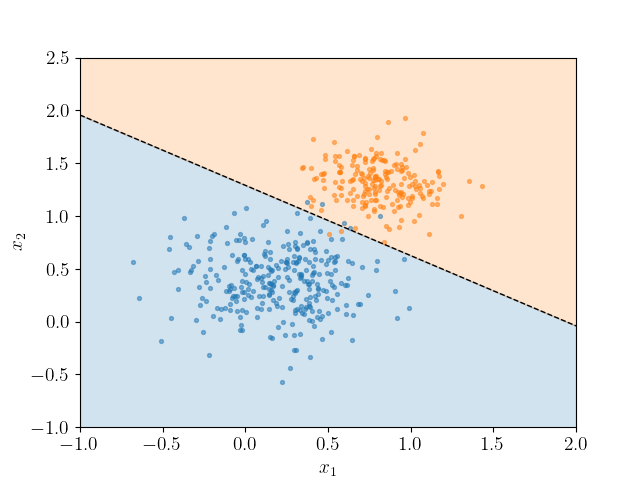
\includegraphics[width=0.7\textwidth]{logistic_regression_boundary.png}
    \captionof{figure}{Hồi quy Logistic học một đường thẳng (hoặc siêu phẳng trong không gian nhiều chiều) để phân chia dữ liệu thành các lớp.}
    \label{fig:logistic_regression_boundary}
\end{center}

\paragraph{Cơ chế hoạt động}
Cho một vector đầu vào $x$ (ví dụ, vector TF-IDF của tài liệu), mô hình thực hiện 2 bước:
\begin{enumerate}
    \item \textbf{Tính toán điểm số tuyến tính (Linear Score):} Mô hình tính một tổng có trọng số của các đặc trưng đầu vào. Mỗi đặc trưng $x_j$ (tương ứng với một từ trong từ vựng) có một trọng số $w_j$.
    $$ z = w_0 + w_1 x_1 + w_2 x_2 + \dots + w_m x_m = w^T x $$
    Trọng số $w_j$ có thể được diễn giải là: một giá trị dương lớn cho thấy sự hiện diện của từ $j$ làm tăng khả năng tài liệu thuộc lớp tích cực, và ngược lại.
    \item \textbf{Ánh xạ qua hàm Sigmoid:} Điểm số $z$ có thể nhận bất kỳ giá trị thực nào. Để biến nó thành một xác suất (nằm trong khoảng [0, 1]), chúng ta đưa nó qua hàm Sigmoid (còn gọi là hàm logistic).
    $$ \sigma(z) = \frac{1}{1 + e^{-z}} $$
\end{enumerate}
Giá trị đầu ra $\sigma(z)$ chính là xác suất dự đoán $P(c=1|d)$.
\paragraph{Huấn luyện bằng Gradient Descent}
Quá trình huấn luyện của Hồi quy Logistic là tìm ra bộ trọng số $w$ tốt nhất để tối thiểu hóa hàm mất mát \textbf{Cross-Entropy} trên toàn bộ tập dữ liệu huấn luyện. Hàm mất mát cho một điểm dữ liệu $(x, y)$ (với $y \in \{0, 1\}$ là nhãn thật) là:
$$ \mathcal{L}(w) = -[y \log(\sigma(w^T x)) + (1-y) \log(1 - \sigma(w^T x))] $$
Gradient của hàm mất mát này theo trọng số $w$ được tính toán, và sau đó thuật toán \textbf{Gradient Descent} (hoặc các biến thể của nó như SGD, Adam) được sử dụng để cập nhật các trọng số $w$ một cách lặp đi lặp lại cho đến khi hội tụ.

\begin{tcolorbox}[
    title=Đánh giá Hồi quy Logistic,
    colback=blue!5!white, colframe=blue!50!black, fonttitle=\bfseries
]
\textbf{Ưu điểm:}
\begin{itemize}
    \item \textbf{Hiệu quả và mạnh mẽ:} Thường cho kết quả tốt hơn Naive Bayes vì nó không có giả định độc lập ngây thơ.
    \item \textbf{Đầu ra là xác suất:} Cung cấp một thước đo độ tin cậy cho dự đoán.
    \item \textbf{Mô hình diễn giải được:} Giống Naive Bayes, có thể kiểm tra các trọng số $w$ để hiểu tầm quan trọng của các từ.
\end{itemize}
\textbf{Nhược điểm:}
\begin{itemize}
    \item \textbf{Bản chất tuyến tính:} Không thể học được các ranh giới quyết định phi tuyến phức tạp. Tuy nhiên, điều này có thể được khắc phục phần nào bằng cách tạo ra các đặc trưng tương tác.
\end{itemize}
\end{tcolorbox}

\subsubsection{Máy Vector Hỗ trợ (Support Vector Machines - SVMs)}
SVM \cite{cortes1995support} là một thuật toán phân loại mạnh mẽ khác, nhưng thay vì tập trung vào xác suất, nó tập trung vào hình học.

\paragraph{Trực giác cốt lõi}
Mục tiêu của SVM là tìm ra một \textbf{siêu phẳng (hyperplane)} phân tách các lớp dữ liệu sao cho \textbf{lề (margin)} -- khoảng cách từ siêu phẳng đến các điểm dữ liệu gần nhất của mỗi lớp -- là \textbf{lớn nhất có thể (maximum margin)}.

\begin{center}
    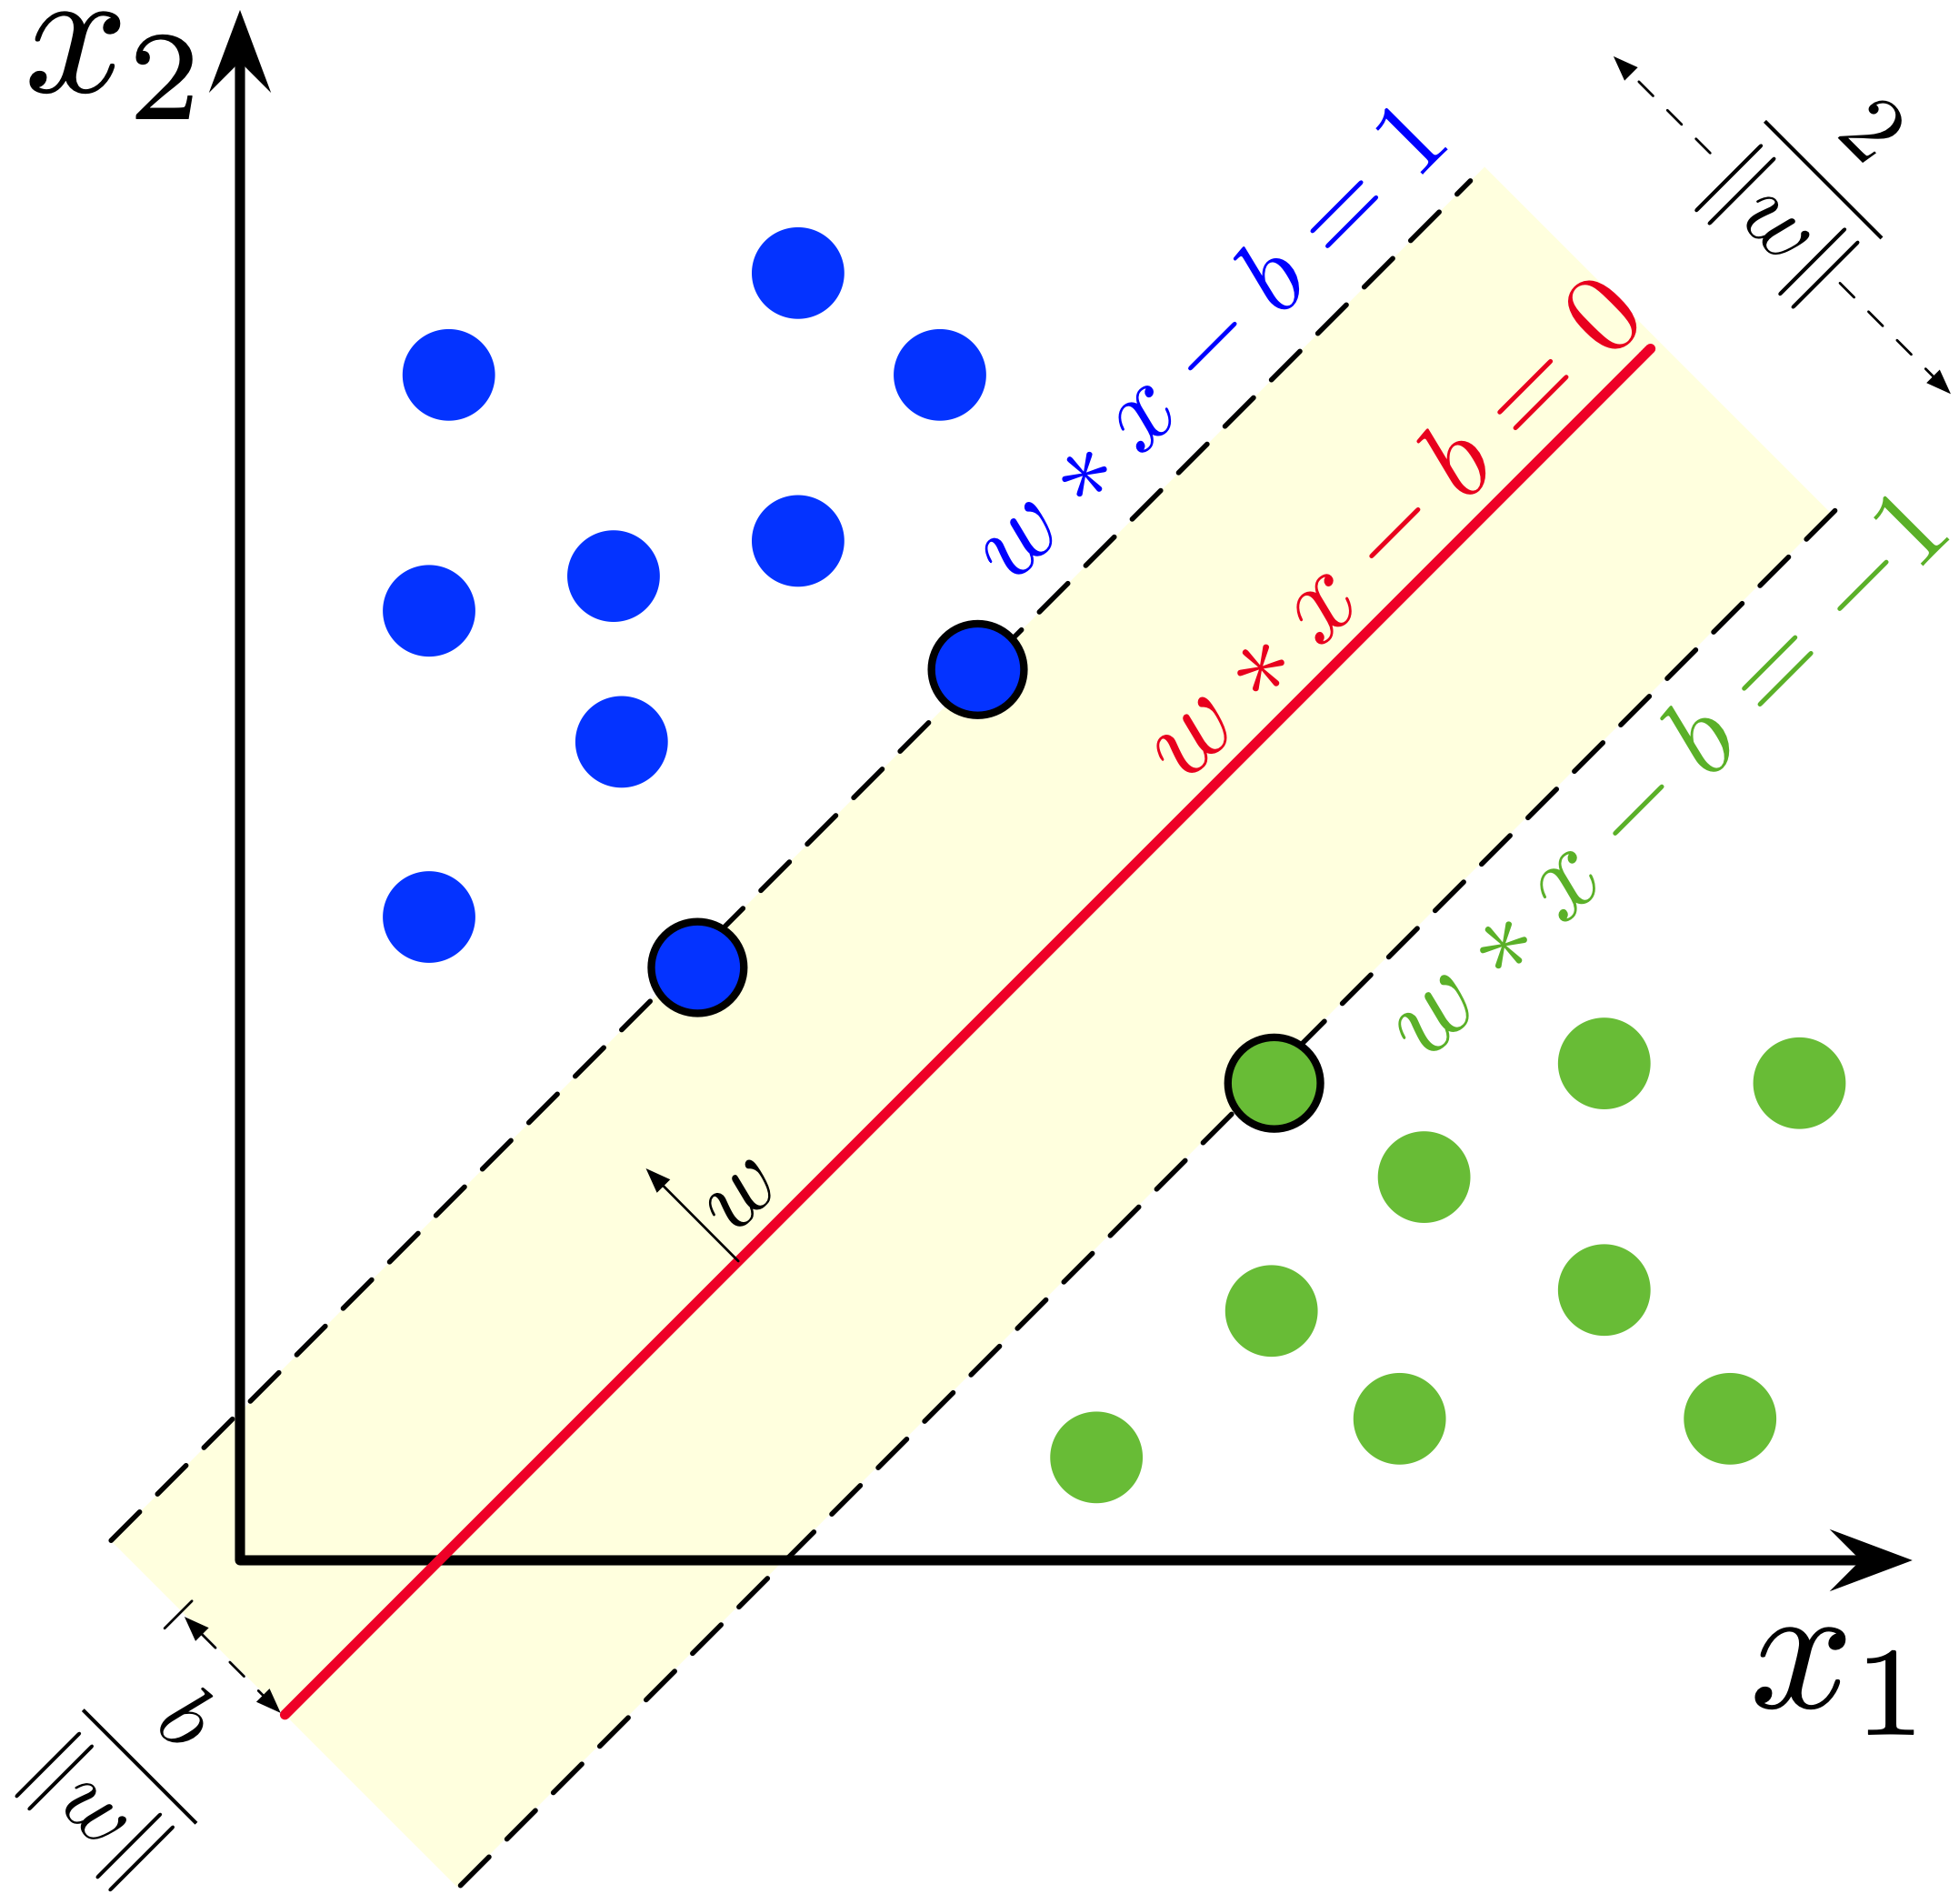
\includegraphics[width=0.7\textwidth]{svm_margin.png}
    \captionof{figure}{SVM tìm siêu phẳng (đường nét đứt) có lề (margin) rộng nhất giữa các lớp. Các điểm nằm trên lề được gọi là các vector hỗ trợ (support vectors).}
    \label{fig:svm_margin}
\end{center}

Việc tối đa hóa lề này giúp mô hình có khả năng tổng quát hóa tốt hơn trên dữ liệu mới, vì ranh giới quyết định ít bị ảnh hưởng bởi nhiễu.

\paragraph{The Kernel Trick}
Điểm mạnh thực sự của SVM nằm ở "thủ thuật kernel" (kernel trick). Nếu dữ liệu không thể phân tách bằng một đường thẳng, SVM có thể sử dụng một hàm kernel (ví dụ: RBF kernel) để ánh xạ dữ liệu lên một không gian nhiều chiều hơn, nơi chúng có thể trở nên phân tách tuyến tính. Điều này cho phép SVM học được các ranh giới quyết định phi tuyến rất phức tạp mà không cần tính toán trực tiếp trong không gian nhiều chiều đó, rất hiệu quả.

\paragraph{Huấn luyện và Hinge Loss}
Quá trình huấn luyện SVM là một bài toán tối ưu hóa nhằm tìm ra siêu phẳng có lề lớn nhất. Điều này được thực hiện bằng cách tối thiểu hóa một hàm mất mát đặc biệt gọi là \textbf{Hinge Loss}:
$$ \mathcal{L}(w) = \max(0, 1 - y_i(w^T x_i - b)) $$
Hàm mất mát này sẽ bằng 0 nếu một điểm dữ liệu nằm đúng phía của lề, và sẽ tăng tuyến tính nếu nó vi phạm lề. Việc tối ưu hóa này thường được giải quyết bằng các phương pháp phức tạp hơn như Quy hoạch toàn phương (Quadratic Programming).

\begin{tcolorbox}[
    title=Đánh giá SVM,
    colback=blue!5!white, colframe=blue!50!black, fonttitle=\bfseries
]
\textbf{Ưu điểm:}
\begin{itemize}
    \item \textbf{Hiệu quả cao trong không gian nhiều chiều:} Rất phù hợp với các vector TF-IDF có số chiều lớn.
    \item \textbf{Học được các ranh giới phi tuyến phức tạp:} Nhờ vào kernel trick.
    \item \textbf{Ít bị quá khớp (overfitting):} Do nguyên lý tối đa hóa lề.
\end{itemize}
\textbf{Nhược điểm:}
\begin{itemize}
    \item \textbf{Chi phí tính toán cao:} Huấn luyện SVM có thể rất chậm trên các bộ dữ liệu lớn.
    \item \textbf{Mô hình hộp đen (Black box):} Việc diễn giải một mô hình SVM với kernel phi tuyến là rất khó.
    \item \textbf{Nhạy cảm với việc lựa chọn kernel và tham số.}
\end{itemize}
\end{tcolorbox}


\subsection{Các mô hình Học chuỗi (Sequence Labeling Models)}
\label{ssec:sequence_models}
Các bài toán như Gán nhãn Từ loại (POS Tagging) hay Nhận dạng Thực thể Tên (NER) không chỉ đơn thuần là phân loại từng từ một cách độc lập. Nhãn của một từ phụ thuộc rất nhiều vào nhãn của các từ xung quanh. Các mô hình học chuỗi được thiết kế để giải quyết vấn đề này.

\subsubsection{Mô hình Markov ẩn (Hidden Markov Models - HMMs)}
HMM \cite{rabiner1989tutorial} là một mô hình sinh kinh điển cho các bài toán gán nhãn chuỗi.

\paragraph{Trực giác cốt lõi}
HMM giả định rằng một chuỗi các quan sát (observations) - tức là các từ trong câu - được "sinh ra" bởi một chuỗi các trạng thái ẩn (hidden states) - tức là các nhãn (ví dụ, các nhãn POS).
Quá trình sinh này tuân theo hai loại xác suất:
\begin{enumerate}
    \item \textbf{Xác suất chuyển trạng thái (Transition Probabilities):} Xác suất chuyển từ một trạng thái ẩn này sang một trạng thái ẩn khác. Ví dụ, $P(\text{Verb}|\text{Noun})$ - xác suất một động từ xuất hiện sau một danh từ. Điều này tuân theo giả định Markov.
    \item \textbf{Xác suất phát sinh (Emission Probabilities):} Xác suất một trạng thái ẩn "sinh ra" một từ quan sát được. Ví dụ, $P(\text{``sách''}|\text{Noun})$ - xác suất từ "sách" được sinh ra khi trạng thái ẩn là Danh từ.
\end{enumerate}

\begin{center}
    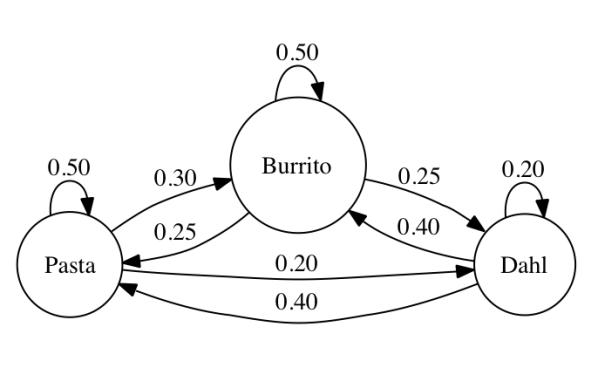
\includegraphics[width=0.8\textwidth]{hmm_diagram.png}
    \captionof{figure}{Sơ đồ một chuỗi Markov (Markov chain) với ba trạng thái: Pasta, Burrito, và Dahl. Các con số biểu thị xác suất chuyển đổi giữa các trạng thái.}
    \label{fig:hmm_diagram}
\end{center}

Nhiệm vụ của HMM là tìm ra chuỗi trạng thái ẩn (chuỗi nhãn) có khả năng nhất đã sinh ra chuỗi các từ quan sát được. Bài toán này được giải quyết hiệu quả bằng một thuật toán quy hoạch động gọi là \textbf{Thuật toán Viterbi (Viterbi Algorithm)}.

\subsubsection{Trường Ngẫu nhiên Có điều kiện (Conditional Random Fields - CRFs)}
CRF, và đặc biệt là Linear-chain CRF, là một cải tiến vượt bậc so với HMM và đã trở thành mô hình thống kê tiêu chuẩn cho các bài toán gán nhãn chuỗi trong nhiều năm.

\paragraph{Sự khác biệt chính với HMM}
HMM là một mô hình sinh, nó mô hình hóa xác suất kết hợp $P(\text{chuỗi quan sát, chuỗi nhãn})$. CRF là một mô hình phân biệt, nó mô hình hóa trực tiếp xác suất có điều kiện $P(\text{chuỗi nhãn}|\text{chuỗi quan sát})$.
Sự thay đổi này mang lại hai lợi thế lớn:
\begin{enumerate}
    \item \textbf{Bỏ giả định độc lập của đặc trưng:} HMM giả định rằng một từ quan sát chỉ phụ thuộc vào trạng thái ẩn hiện tại. CRF không có giả định này. Nó có thể sử dụng một loạt các đặc trưng phức tạp của chuỗi đầu vào, ví dụ: "từ hiện tại có viết hoa không?", "hậu tố của từ hiện tại là gì?", "từ trước đó là gì?". Điều này làm cho CRF linh hoạt và mạnh mẽ hơn nhiều.
    \item \textbf{Tránh tính toán $P(\text{chuỗi quan sát})$:} Việc mô hình hóa xác suất của chuỗi quan sát là rất khó, CRF đã loại bỏ được gánh nặng này.
\end{enumerate}

\paragraph{Trực giác cốt lõi của CRF}
Thay vì tính toán các xác suất chuyển và phát sinh riêng lẻ, một CRF gán một điểm số (score) cho mỗi cặp (chuỗi quan sát, chuỗi nhãn) dựa trên một tổ hợp tuyến tính của các hàm đặc trưng (feature functions). Các hàm đặc trưng này có thể bắt các mối quan hệ phức tạp giữa các từ và nhãn. Sau đó, nó sử dụng một hàm chuẩn hóa (tương tự softmax) trên toàn bộ các chuỗi nhãn có thể có để biến điểm số thành xác suất. Nhiệm vụ cũng là tìm ra chuỗi nhãn có xác suất (điểm số) cao nhất, và cũng thường được giải bằng thuật toán Viterbi.

\begin{tcolorbox}[
    title=So sánh HMM và CRF,
    colback=green!5!white, colframe=green!60!black, fonttitle=\bfseries
]
\begin{tabular}{p{0.45\linewidth} | p{0.45\linewidth}}
    \textbf{Hidden Markov Models (HMM)} & \textbf{Conditional Random Fields (CRF)} \\
    \hline
    Mô hình \textbf{sinh} (Generative) & Mô hình \textbf{phân biệt} (Discriminative) \\
    \hline
    Mô hình hóa $P(\text{observations, labels})$ & Mô hình hóa $P(\text{labels | observations})$ \\
    \hline
    Giả định các quan sát độc lập có điều kiện & Không có giả định độc lập, cho phép các đặc trưng chồng chéo, phức tạp. \\
    \hline
    Huấn luyện nhanh hơn & Huấn luyện chậm hơn (cần các thuật toán lặp) \\
    \hline
    Thường cho hiệu năng thấp hơn & Thường cho hiệu năng \textbf{vượt trội}, là state-of-the-art trong kỷ nguyên thống kê. \\
\end{tabular}
\end{tcolorbox}